\chapter{Formative Studies}
\label{sec:formative}

The previous chapter covered background literature and prior work by
other researchers. This chapter presents original work studying design
culture, specifically related to rapid fabrication with laser cutters.

This chapter presents three studies. First, I give observations of
people working at a professional design studio. It gives a firsthand
account of processes that real designers use when practicing their
craft. Second, to better understand the tasks and problems designers
face when designing for laser cutters, I conducted two related
formative studies. I interviewed people with experience designing
laser cut artifacts and watched them work. In addition, I surveyed and
analyzed laser-cut items found on community web sites to identify
common features.

\section{Tiny Ethnography}
\label{sec:formative-tiny-ethnography}

I arranged to ``be a fly on the wall'' at a MAYA Design,
well-respected design firm in the Pittsburgh area. This was done to
observe how designers work. I spent about twenty hours at the company
observing and interviewing designers who work there. This study was
inspired by Bucciarelli's ethnographies of
engineers~\cite{bucciarelli-designing-engineers}. While this work
pre-dates my focus on design for laser cutters, it does provide a
solid connection between my narrow topic and the broader context of
design practice.

A professional studio is notably different from an educational design
studio. For example, companies face many issues that are not generally
present in an academic institution. These include billable hours,
interacting with paying customers, significant differences in age and
experience level of collaborators, and so on.

This company's culture places high value on collaborative whiteboard
sessions. At any time, the majority of the whiteboard surfaces
throughout the office have some sort of scribbling on them. Most
whiteboard sessions were by two or more people gathered in
conversation. The scribbles served to represent objects that are
sometimes labeled with markers, but usually just described
verbally. In this way, collaborative whiteboard drawings are
multi-modal design artifacts, because part of their value is static
(the sketch), while another part is transient (the
conversation)~\cite{ju-navigator}. Whiteboard sessions are consistent
with Ferguson's \textit{talking sketches}~\cite{ferguson-engineering}.

Four of the five designers I interviewed showed me their paper
sketches. About half of these drawings were made when the designer was
alone (Ferguson's \textit{thinking sketch}), and the rest resulted
from collaborative sessions like the whiteboard events described
above. Some paper sketches were diagrammatic (using formal or
semi-formal notation), while others were renderings of some physical
object like a building or electronic gadget. Interestingly, those same
designers were less inclined to show computational models (like
Illustrator files) because they felt the sketches contained the
``real'' work.

While designers typically did not volunteer to show computational
artifacts, they were inclined to show me printed versions of their
computational models. Nearly all of these printed pages were annotated
with handwriting and sketches, sometimes by more than one person. They
use a process of iterating between virtual and paper representations
of their work. The designers would edit a computational model with a
high-functionality application such as Photoshop, then print a paper
copy for personal or group use. Then they would draw or write directly
on that page as they explored variations or made refinements. If a
paper-based editing session was useful, the designers would then
manually transfer these changes back into their application. The
process of printing, editing, and manually merging changes was
common. This pattern recurs in the following section on laser cutter
users.

\section{Interviews}
\label{sec:formative-interviews}

\begin{figure}[t]
  \centering
  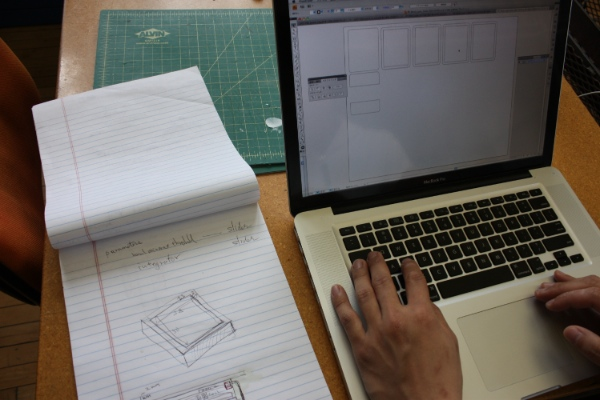
\includegraphics[width=0.7\linewidth]{img/translate-sketch-to-computer.jpg}
  \caption[Translating paper sketch to computer model]{A common step
    of designing for laser cutters: translating a hand-made sketch to
    a computer modeling tool. The sketch includes a perspective
    drawing of the desired result, and 2D diagrams of individual parts
    with key dimensions indicated.}
  \label{fig:translate}
\end{figure}


Six designers were interviewed from different backgrounds, including
mechanical engineering, graphic design, and architecture. This was
done to learn about their work practices and to understand how they
use their tools. All had experience designing objects to be made with
a laser cutter.

Each session lasted approximately one hour, split evenly between an
interview and using software. Meetings took place in participant
workplaces, where they were asked to describe their design process and
to show sketches, demonstrations, or videos of their work. Although
there were differences in their process, each followed the same
overall pattern.

The designers all said they began by thinking about a problem and
sketching on paper. They made drawings to think about how to ``frame''
the project (what it is for). Other sketches helped reason about how
to make it (how it works and fits together). Some designers explicitly
noted that sketching is a necessary part of the process: they could
not move forward without making freehand drawings. Only after the idea
was well-formed were they ready to translate their hand-made sketch
into a computer model (Figure~\ref{fig:translate}).

After the interview, participants were asked to copy the sketch shown
in Figure~\ref{fig:interview-sketch} using a software tool of their
choice. This was done to learn what problems people encountered when
executing the common task of translating a sketch to a computer model.


\begin{figure}[t]
\centering \subfloat[We asked users to replicate this sketched part.]
           {
  \label{fig:interview-sketch-1} 
  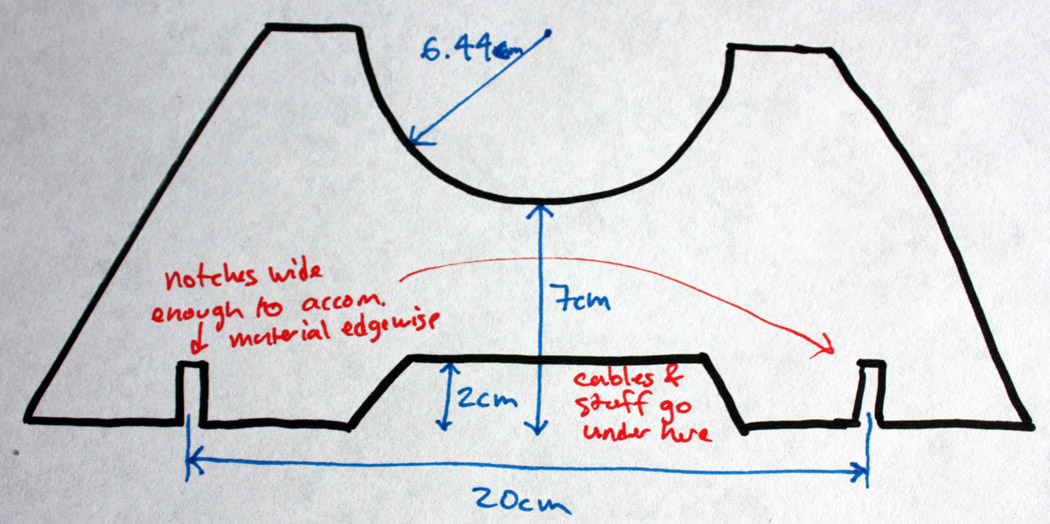
\includegraphics[width=0.7\linewidth]{img/laser-me-1.jpg}
}

\subfloat[Drawing of the part in context.] {
    \label{fig:interview-sketch-2}
    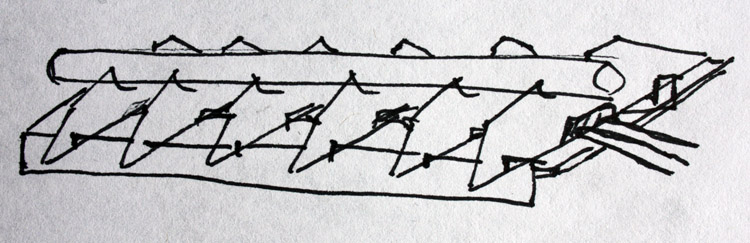
\includegraphics[width=0.7\linewidth]{img/laser-me-2.jpg}
}
\caption[Sketch from designer interview activity]{We asked
  participants to model the part at the top using a software of their
  choice.}
\label{fig:interview-sketch}
\end{figure}


Five participants chose to implement the sketch with Illustrator; one
chose Rhino. All users were comfortable with their tools, but none
were experts. Every designer's strategy involved common activities:
creating and editing boundaries, aligning or snapping items, using
guide lines or reference points, measuring distances, specifying or
changing lengths and angles, and creating finished ``cut files'' to
send to the laser cutter. They also engaged in the usual interaction
management tasks---selecting and deselecting on-screen elements, and
view port management such as zooming and panning.

Participants spent a good deal of time on operating overhead
(approximately 50\%, or about 15 minutes per interview). This included
searching for appropriate tools for the next task, and recovering from
errors. Consider the example of one designer who was an experienced
Illustrator user. He was aware of the ``Path Finder'' tool and wanted
to use it. He slowly searched the program's menu structure and hovered
over toolbar buttons to read tool tips. Upon finding the Path Finder,
he invoked various functions, using the keyboard shortcut (Control-Z)
to undo after each failed attempt, as he searched for the correct mode
within the subcommand palette. This process lasted approximately 80
seconds.

Occasionally participants used features in unorthodox ways. For
example, to remove an unwanted segment of a polyline, one participant
(a graphic designer) created an opaque white rectangle to obscure it,
rather than erase it. (``Don't tell anyone I did this'', he said).

Similar episodes are common: a person \textit{should} know the
`correct' action, but takes an alternate approach. Although the
alternative achieves the intended effect, it might be less efficient
(more operations, longer execution time) or introduce unwanted
complexity (e.g. the white rectangle).

In short, most common tasks and problems belong to three main groups:

\begin{itemize}
\item \textit{Defining geometry:} Creating/editing boundaries,
  aligning items, creating and using guide lines or reference points,
  measuring distances, and specifying lengths or angles.
\item \textit{Managing the editing tool:} Selecting/deselecting
  objects, view port management, finding and entering tool modes, and
  recovering from errors.
\item \textit{Cut file:} Finalizing the cut file by creating copies of
  items when more than one is needed, and positioning stencils.
\end{itemize}

\section{Artifact Analysis}
\label{sec:formative-artifact}

The formative study of work practices from the previous section helps
us understand \textit{how} people create laser cut items. To learn
more about the characteristics of those objects (\textit{what} people
create), I analyzed finished items from two web-based communities of
laser cutter users.

Many users are motivated by the opportunity to share their work with
others. Ponoko and Thingiverse are two currently popular web sites for
selling or sharing items that can be made with rapid fabrication
machines. In early 2012, Ponoko offers thousands of user-designed
items for sale, mostly produced by laser cutting. Thingiverse is a
warehouse of digital models of 3D-printable objects and designs for
laser cutters. From these two sites I selected a total of 55 laser-cut
designs. On Ponoko, the most recent 45 laser cut items were chosen.
On Thingiverse, ten objects with the ``laser cutter'' were
selected. Figure~\ref{fig:ponoko} summarizes the feature analysis of
these 55 projects.

\begin{figure}[t]
  \centering
  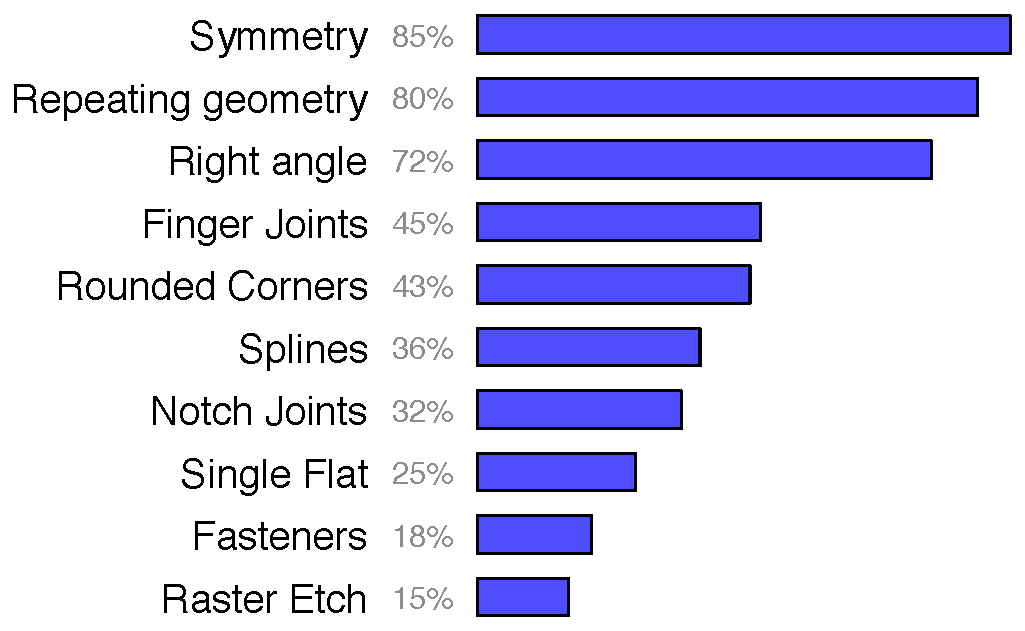
\includegraphics[width=0.6\linewidth]{img/ponoko-graph.pdf}
  \caption[Feature Analysis of Laser Cut Items]{Frequency of features
    of 55 laser-cut designs found on Ponoko and Thingiverse.}
  \label{fig:ponoko}
\end{figure}


Each project was characterized using ten properties, based on my own
experience designing objects for laser cutters, as well as
observations from the formative study. They are:

\begin{itemize}
\item \textit{Symmetry}: Radial/linear symmetry is present.
\item \textit{Repeating geometry}: Line work is repeated several times.
\item \textit{Right Angle}: Edges meet at 90-degree angles.
\item \textit{Notch and Finger Joints}: Parts join in one of the ways
  shown in Figure~\ref{fig:joint}.
\item \textit{Rounded Corners}: Right-angle corners are slightly blunt.
\item \textit{Splines}: Curved line work (not counting rounded corners).
\item \textit{Single Flat}: The project is composed of a single, flat
  piece of material (e.g. a coaster).
\item \textit{Fasteners}: Use of glue, screws, or bolts.
\item \textit{Raster etch}: Patterns like words and images are etched
  in material.
\end{itemize}

This list of properties helped inform what SIMI should (and should
not) do. However, it is important to note that the features provided
by SIMI was not explicitly determined by this analysis; rather, the
most common features were favored. Rounded corners, for example, were
not included in SIMI because that feature did not support a
substantially greater outcome. By contrast, Symmetry was not
explicitly supported (e.g. by a 'mirror' tool or similar) but was
implicitly made possible with a combination of angle and length
constraints.

\begin{figure}[b]
\centering 
\subfloat[Notch joints.] {
  \label{fig:joint-notch} 
  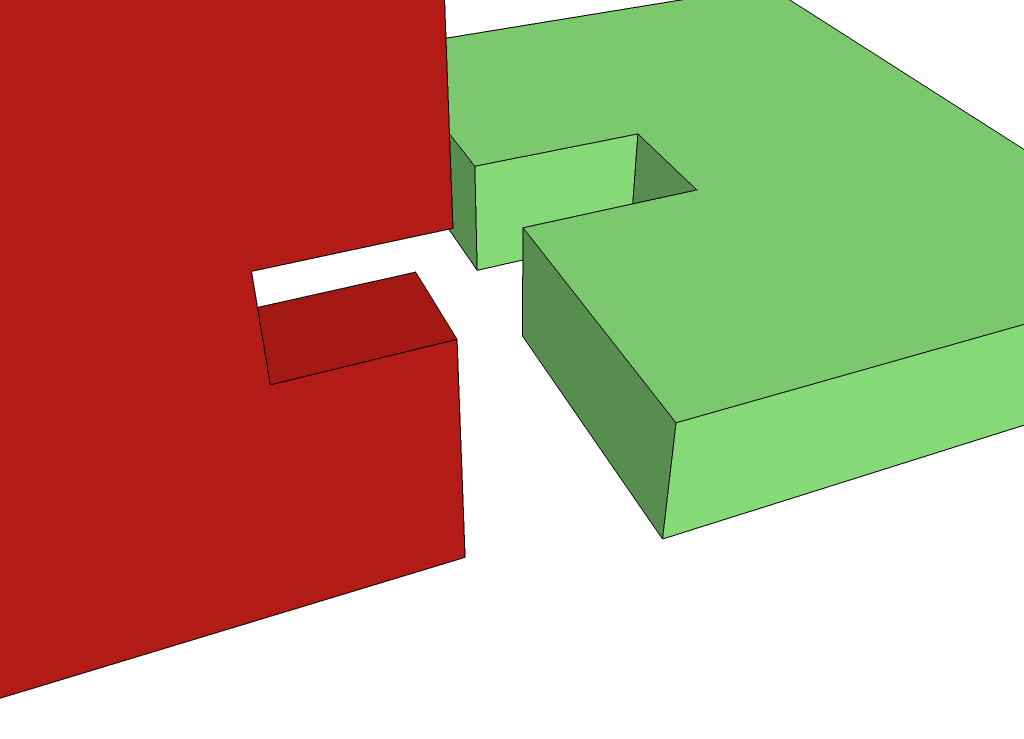
\includegraphics[width=0.3\linewidth]{img/joint-notch.png}
}
\subfloat[Finger (box) joints.] {
    \label{fig:joint-finger}
    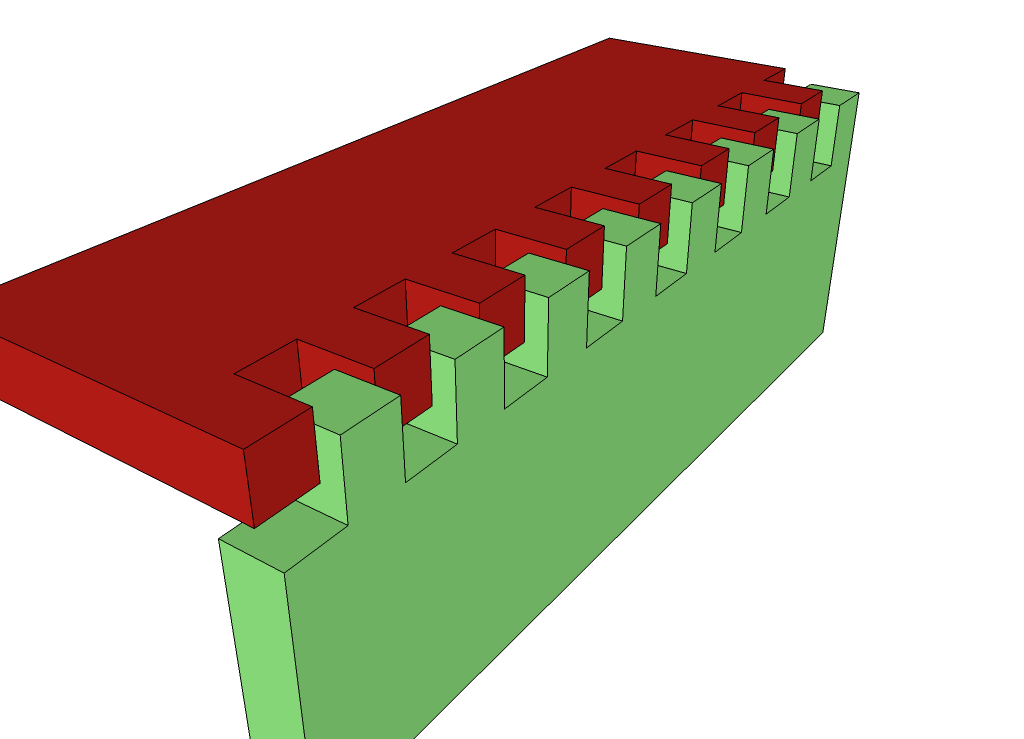
\includegraphics[width=0.3\linewidth]{img/joint-finger.png}
}
\caption[Two common notch types]{Two common methods to join
  parts. Notch joints are used when parts intersect along part
  midsections; finger joints (box joints) join parts along edges.}
\label{fig:joint}
\end{figure}





